\documentclass[11pt]{article}
\usepackage[a4paper,margin=2.4cm]{geometry}
\usepackage{booktabs,graphicx,amsmath,hyperref,xcolor}
\hypersetup{colorlinks,linkcolor=blue!50!black,citecolor=blue!50!black,urlcolor=blue!50!black}
\usepackage[numbers,sort&compress]{natbib}

\title{What Does Hybrid Post-Quantum Key Exchange Cost a Microservice?\\
\large Measuring X25519MLKEM768 in Go's Standard TLS Stack}
\author{Mithil Nagabathula\\University of East London\\\texttt{mithilnishu2000@gmail.com}}
\date{October 2026}

\begin{document}
\maketitle
\sloppy

\begin{abstract}
Hybrid post-quantum key exchange protects TLS traffic recorded today against decryption by a future quantum computer, and Go 1.24
enables X25519MLKEM768 by default. Service-to-service traffic inside a platform is where adoption is easiest and where the cost is
paid most often. We measure that cost in Go's standard library with no third-party code: the key-exchange primitives, 28 handshake
configurations across four certificate types, with and without mutual TLS and session resumption, and the bytes in every flight. The
hybrid group added 2{,}311 bytes to a mutual-TLS handshake (1{,}721 to 4{,}032) and, with ECDSA certificates, 47\% to server CPU time per
full handshake (807 to 1{,}185 \(\mu\)s on our test machine) and 56\% on the client. With RSA-2048 certificates the relative overhead fell
to 14\% because the signature dominates. The ClientHello grew from 224 to 1{,}446 bytes, still one segment on Ethernet but two behind a
typical VPN tunnel or at the IPv6 minimum MTU; resumed handshakes still pay the key exchange. A hybrid-capable client talking to a
classical server pays the larger ClientHello for no benefit. In a simple network model the hybrid adds about 1 ms inside a data
centre, 4\% on broadband and 17--21\% on 1 Mbit/s and slower links. For most microservice traffic, connection reuse matters far more than
the choice of key-exchange group.
\end{abstract}

\section{Introduction}
Data encrypted today with elliptic-curve key exchange can be recorded and decrypted later if a cryptographically relevant quantum
computer is built, the ``harvest now, decrypt later'' risk \cite{mosca2018}. NIST standardised ML-KEM \cite{fips203} and has set
deadlines to retire quantum-vulnerable public-key algorithms \cite{nistir8547}. The interim answer in TLS 1.3 \cite{rfc8446} is hybrid key
exchange \cite{hybriddesign}: the client and server combine X25519 with ML-KEM-768 in a single group, X25519MLKEM768 \cite{ecdhemlkem}, so
the session is secure if either component is.

Earlier benchmarks studied post-quantum TLS with research libraries \cite{paquin2020,sikeridis2020}. Hybrid key exchange is now in
production stacks: Go 1.24 enables it by default \cite{go124}. Engineers deciding whether to keep it on for internal services need
numbers from the stack they run, for the configurations they use: mutual TLS, ECDSA or RSA certificates, session resumption, and a
mixture of updated and old peers. This paper provides them.

\section{Method}
\paragraph{Implementation.} A single Go program (Go 1.24.7, standard library only) times the primitives with \texttt{crypto/ecdh} and
\texttt{crypto/mlkem}, and runs TLS 1.3 handshakes between two separate processes over loopback TCP with \texttt{crypto/tls}. The server
accepts a configured number of connections, completes each handshake, reads one application byte, and reports its own process CPU time
(user plus system, from \texttt{getrusage}) per handshake. The client reports its CPU time the same way. A wrapper around the server's
connection records the size of every read and write, from which we obtain the bytes in each flight.

\paragraph{Configurations.} Server groups X25519, P-256 and X25519MLKEM768; the hybrid client also offers an X25519 share, which is Go's
default behaviour. Certificates: ECDSA P-256, Ed25519, RSA-2048, RSA-3072. Each with and without mutual TLS (client certificates). Plus
session resumption (PSK with key exchange), a hybrid-capable client against a classical server, and a hybrid-only client. Each
configuration ran 7 times with 300 handshakes per run; we report medians across runs.

\paragraph{Environment and caveats.} Measurements ran on a shared 2-vCPU cloud virtual machine. Absolute CPU times are therefore higher
than on dedicated servers and include TCP connection handling; relative differences between groups on the same machine are the
meaningful quantity, and we report interquartile ranges. Network effects are modelled rather than emulated, because the environment
provided no traffic shaping.

\section{Results}
\subsection{Primitives}
\begin{table}[t]
\centering
\caption{Key-exchange primitives in Go 1.24 (\texttt{crypto/ecdh}, \texttt{crypto/mlkem}), 15 repetitions of 2{,}000 operations. Public values: X25519 32 bytes, P-256 65 bytes, ML-KEM-768 encapsulation key 1,184 bytes and ciphertext 1,088 bytes.}
\label{tab:prims}
\small
\begin{tabular}{lrr}
\toprule
Operation & Median ($\mu$s) & IQR ($\mu$s) \\
\midrule
X25519 keygen & 72.2 & 8.6 \\
X25519 shared secret & 73.9 & 12.1 \\
P-256 keygen & 20.0 & 1.6 \\
P-256 shared secret & 80.8 & 13.1 \\
ML-KEM-768 keygen & 88.0 & 8.0 \\
ML-KEM-768 encapsulate & 90.1 & 8.1 \\
ML-KEM-768 decapsulate & 121.7 & 8.0 \\
ML-KEM-1024 keygen & 127.0 & 11.3 \\
ML-KEM-1024 encapsulate & 151.1 & 17.2 \\
ML-KEM-1024 decapsulate & 192.5 & 11.3 \\
\bottomrule
\end{tabular}
\end{table}

ML-KEM-768 encapsulation and decapsulation cost 1.2 and 1.6 times one X25519 shared-secret computation on this machine (Table~\ref{tab:prims}). In a
hybrid handshake the client generates an ML-KEM key pair and decapsulates, and the server encapsulates, on top of the X25519 work, so the
expected extra CPU is roughly one X25519-equivalent operation per side, plus the cost of handling larger messages.

\subsection{Handshakes}
\begin{table*}[t]
\centering
\caption{Full TLS 1.3 handshakes on loopback, X25519 against X25519MLKEM768 (the hybrid client also offers an X25519 share, Go's default). CPU is median process CPU time per handshake over 7 runs of 300 handshakes; bytes are the handshake records in both directions. Pairs are X25519 / X25519MLKEM768.}
\label{tab:hs}
\small
\begin{tabular}{llrrrr}
\toprule
Certificate & mTLS & Server CPU, $\mu$s & $\Delta$ server & Client CPU, $\mu$s & Bytes \\
\midrule
ECDSA-P256 & no & 542 / 831 & +53\% & 749 / 1177 & 1,076 / 3,387 \\
ECDSA-P256 & yes & 807 / 1185 & +47\% & 943 / 1475 & 1,721 / 4,032 \\
Ed25519 & no & 613 / 706 & +15\% & 832 / 1041 & 1,006 / 3,316 \\
Ed25519 & yes & 781 / 910 & +16\% & 942 / 1133 & 1,582 / 3,892 \\
RSA-2048 & no & 2669 / 3045 & +14\% & 938 / 1446 & 1,658 / 3,968 \\
RSA-2048 & yes & 3059 / 3187 & +4\% & 3338 / 3431 & 2,886 / 5,196 \\
RSA-3072 & no & 6014 / 6266 & +4\% & 1440 / 1799 & 2,042 / 4,352 \\
RSA-3072 & yes & 7486 / 7526 & +1\% & 7900 / 7926 & 3,654 / 5,964 \\
\bottomrule
\end{tabular}
\end{table*}


\paragraph{CPU.} With ECDSA certificates, the hybrid group raised server CPU per full handshake by 53\% without client certificates and
47\% with them, and client CPU by 57\% and 56\% (Table~\ref{tab:hs}). The relative cost depended strongly on the certificate: with Ed25519
it was 15\% on the server, with RSA-2048 14\%, and with RSA-3072 4\%, because RSA signing dominates. On this machine a single core could
complete about 1{,}240 mutual-TLS handshakes per second with X25519 and about 840 with the hybrid group.

\paragraph{Bytes.} The hybrid ClientHello grew from 224 to 1{,}446 bytes, and the server's first flight from 864 to 1{,}953 bytes in mutual
TLS (Figure~\ref{fig:flights}). A whole mutual-TLS handshake grew from 1{,}721 to 4{,}032 bytes. A hybrid-only client, which does not also
offer an X25519 share, saved 38 bytes.

\begin{figure}[t]
  \centering
  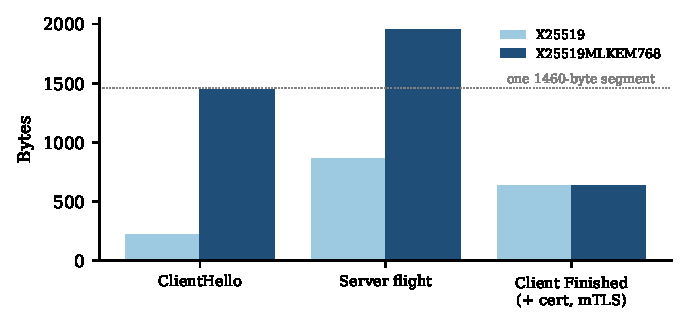
\includegraphics[width=0.7\linewidth]{figures/flights.pdf}
  \caption{Bytes per flight in a mutual-TLS handshake with ECDSA certificates.}
  \label{fig:flights}
\end{figure}

\paragraph{Packets.} The hybrid ClientHello still fits in one TCP segment with Ethernet's 1{,}460-byte MSS, by 14 bytes. Behind an IPsec or
WireGuard tunnel (MSS about 1{,}380) or at the IPv6 minimum MTU (MSS 1{,}220) it needs two segments, and a resumed hybrid ClientHello,
carrying a session ticket as well, needs two everywhere (2{,}026 bytes). Two-segment ClientHellos are handled by compliant stacks but are
the case that some middleboxes have historically mishandled.

\paragraph{Resumption does not avoid the cost.} Go resumes sessions with PSK plus a fresh key exchange, so resumed hybrid handshakes still
paid the ML-KEM work: 790 against 517 \(\mu\)s of server CPU for X25519. Resumption saved the certificate signature and verification, not
the key exchange.

\paragraph{Mixed estates.} A hybrid-capable client connecting to a classical-only server negotiated X25519 without a retry but sent the
1{,}446-byte ClientHello every time. During a migration, clients updated before servers pay the byte cost without the protection.

\subsection{Network model}
\begin{table}[t]
\centering
\caption{Modelled cost of a full mTLS handshake (ECDSA certificates): one round trip, serialisation of the measured handshake bytes, and the measured CPU time on both sides. Only one round trip is needed in every case: the largest flight (1,953 bytes) fits well within a 10-segment initial congestion window.}
\label{tab:net}
\small
\setlength{\tabcolsep}{4pt}
\begin{tabular}{lrrrrr}
\toprule
Environment & Bandwidth & RTT (ms) & Classical (ms) & Added by hybrid (ms) & Relative \\
\midrule
Same host / data centre & 10000 Mbit/s & 0.1 & 1.85 & 0.91 & +49\% \\
Cross-zone & 1000 Mbit/s & 1 & 2.76 & 0.93 & +34\% \\
Internet, broadband & 50 Mbit/s & 30 & 32.03 & 1.28 & +4\% \\
Mobile, constrained & 1 Mbit/s & 100 & 115.52 & 19.40 & +17\% \\
Low-power IoT link & 0.25 Mbit/s & 300 & 356.82 & 74.86 & +21\% \\
\bottomrule
\end{tabular}
\end{table}

Table~\ref{tab:net} combines one round trip, serialisation of the measured bytes and the measured CPU time. Every flight fits within a
10-segment initial congestion window \cite{rfc6928}, so the hybrid never adds a round trip. Inside a data centre the added time, about
0.9~ms, is almost all CPU and is large in relative terms (34--49\%) only because the classical handshake is so cheap. On broadband the
hybrid adds 4\%. On 1 Mbit/s and 250 kbit/s links the extra 2.3~kB costs 19--75~ms, 17--21\% of the handshake.

\section{Discussion}
For microservices, the result to act on is that the hybrid cost is paid per handshake. A service that reuses connections, as HTTP/2 and
gRPC clients and most connection pools do, pays it once per connection lifetime, and its share of request latency becomes negligible.
Services that open a connection per request, or that are fronted by short-lived serverless instances, pay it every time and should
measure it. Certificate choice moves the relative cost more than the key exchange does: a fleet on RSA-3072 will barely notice the
hybrid, while a fleet on Ed25519 or ECDSA will see the CPU per handshake rise by a sixth to a half.

Three practical points follow. (1) Upgrade servers before or with clients, since hybrid clients talking to classical servers pay the
bytes for nothing. (2) Check MTU on tunnelled paths, where the ClientHello now spans two packets. (3) Keep the hybrid on for long-lived
internal connections: the cost is small once amortised, and internal traffic is exactly what a harvest-now attacker inside a network
would record.

\paragraph{Limitations.} One machine, one language runtime and loopback networking; a shared virtual machine inflates absolute CPU times.
The network model ignores loss, congestion and middlebox behaviour. Post-quantum signatures, which would change certificate sizes and
signature costs far more than ML-KEM changes key exchange, were not tested because Go's standard library does not yet provide them for
TLS.

\section{Conclusion}
In Go's standard TLS stack, X25519MLKEM768 added about 2.3~kB and, with elliptic-curve certificates, about half again the CPU time of a
full handshake, with no extra round trip. With connection reuse that is a small price for protection against recorded-traffic
decryption.

\paragraph{Reproducibility.} The benchmark is one Go program with no dependencies; code and results will be released at
\newline\url{https://github.com/mithil2k2000-tech/pq-tls-microservices}.

\paragraph{Use of AI tools.} An AI assistant (Claude, Anthropic) helped write the benchmark code and draft text. The author designed the
study, reviewed the code and results, and takes responsibility for the content.

\bibliographystyle{plainnat}
\bibliography{refs}
\end{document}
